\documentclass{article}
\usepackage{amsmath}
\usepackage{minted}
\usepackage[a4paper, margin=1in]{geometry}
\usepackage{graphicx}
\usepackage{hyperref}
\usepackage{fancyhdr}
\usepackage{booktabs}
\usepackage{listings}
\usepackage{caption}
\usepackage{subcaption}
\usepackage[toc,page]{appendix}
\usepackage[dvipsnames]{xcolor}
\usepackage[sorting=none]{biblatex}
\addbibresource{references.bib} 
\pagestyle{fancy}
\fancyhf{}
\renewcommand{\headrulewidth}{0pt}
\renewcommand{\footrulewidth}{1pt}
\fancyfoot[C]{\thepage}

\begin{document}
\begin{center}
{\textcolor{RedOrange}{Applied Machine Learning}} \\
\vspace{0.5em}
\text{\LARGE Homework 11} \\
\vspace{1em}
\href{mailto:amk23j@fsu.edu}{Anand Kamble}\\
\text{Department of Computer Science} \\
\text{Florida State University}
\end{center}
\noindent\hrulefill

\section*{Principal Component Analysis (PCA) on Horse Images}

In this report, we perform Principal Component Analysis (PCA) on a set of horse images and a single bird image. The PCA is performed using Singular Value Decomposition (SVD) of the centered horse images. We explore various components of PCA such as discarding certain principal components, projecting data onto principal components, reconstructing images using different numbers of principal components, and analyzing distances in PCA-transformed spaces.

\subsection*{Approach and Implementation}

\subsubsection*{Data Loading and Normalization}

We load a total of 327 horse images and a single bird image, converting them to grayscale and flattening them into vectors. Pixel values are normalized to the range [0,1]:

\begin{minted}[fontsize=\small,frame=single]{python}
import numpy as np
import matplotlib.pyplot as plt
from PIL import Image
import glob

horse_images_path = sorted(glob.glob('horses/*.png'))
horses = []
for img_path in horse_images_path:
    img = Image.open(img_path).convert('L')
    img_array = np.asarray(img, dtype=float) / 255.0  # Normalize pixel values to [0,1]
    horses.append(img_array.flatten())
horses = np.array(horses)  # shape: (327, 128*128)

bird_image_path = 'bird.png'
bird_img = Image.open(bird_image_path).convert('L')
bird_array = np.asarray(bird_img, dtype=float) / 255.0
bird_vector = bird_array.flatten()  # Flatten bird image
\end{minted}

\subsubsection*{Computing Mean and Centering Horse Data}

We compute the mean of the horse images and center them by subtracting this mean from each image vector. This step is crucial for PCA:

\begin{minted}[fontsize=\small,frame=single]{python}
mean_horse = np.mean(horses, axis=0)

horses_centered = horses - mean_horse
\end{minted}

\subsubsection*{Performing PCA using SVD}

Principal Component Analysis is performed by computing the Singular Value Decomposition (SVD) of the centered horse data. The principal components (PCs) are derived from the singular vectors:

\begin{minted}[fontsize=\small,frame=single]{python}
U, S, VT = np.linalg.svd(horses_centered, full_matrices=False)
V = VT.T  # Principal components (eigenvectors)
\end{minted}

\subsubsection*{a) Discarding the Two Largest Singular Values}

We visualize the singular values after discarding the two largest ones, to focus on the smaller and subsequent components:

\begin{minted}[fontsize=\small,frame=single]{python}
remaining_singular_values = S[2:]  # discard the first two largest singular values
plt.figure(figsize=(6,4))
plt.plot(remaining_singular_values, marker='o')
plt.title('Remaining Singular Values (Sorted in Decreasing Order)')
plt.xlabel('Index')
plt.ylabel('Singular Value')
plt.show()
\end{minted}

\begin{figure}[h]
    \centering
    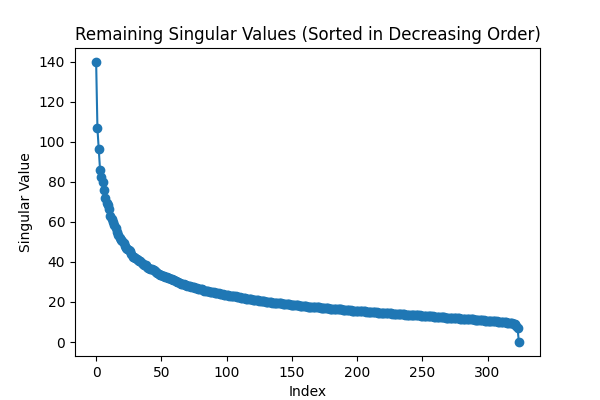
\includegraphics[width=.6\textwidth]{remaining_singular_values.png}
    \caption{Remaining Singular Values After Discarding the Two Largest}
    \label{fig:remaining_singular_values}
\end{figure}

\subsubsection*{b) Projecting the Horses onto the First Two Principal Components}

We project the centered horse images onto the first two principal components (PC1 and PC2) and plot them to visualize the data distribution in the new 2D feature space:

\begin{minted}[fontsize=\small,frame=single]{python}
pcs = V[:, :2]  # first two principal components
horse_projections = horses_centered.dot(pcs)

plt.figure(figsize=(6,4))
plt.scatter(horse_projections[:,0], horse_projections[:,1], c='black', label='Horses')
plt.title('Projection of Horses onto First 2 PCs')
plt.xlabel('PC1')
plt.ylabel('PC2')
plt.legend()
plt.show()
\end{minted}

The output is shown in \ref{fig:horse_projections}

\begin{figure}[ht]
    \centering
    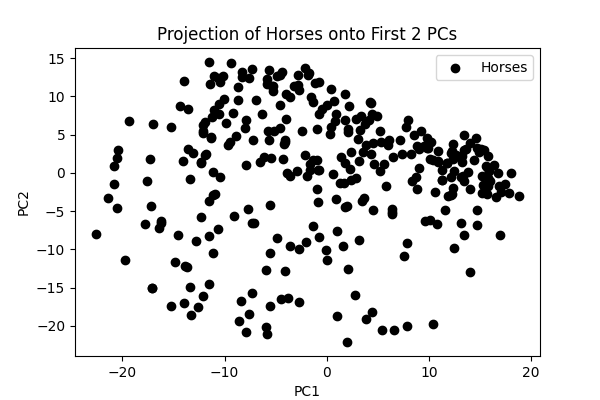
\includegraphics[width=.6\textwidth]{horse_projections.png}
    \caption{Horse Images Projected onto the First Two Principal Components}
    \label{fig:horse_projections}
\end{figure}
\newpage
\subsubsection*{c) Plotting Bird Projection Alongside Horse Projections}

We project the bird image onto the same two principal components (PC1 and PC2) derived from the horse images and plot it alongside the horse projections:

\begin{minted}[fontsize=\small,frame=single]{python}projection in red 'x'
bird_centered = bird_vector - mean_horse
bird_projection = bird_centered.dot(pcs)

plt.figure(figsize=(6,4))
plt.scatter(horse_projections[:,0], horse_projections[:,1], c='black', label='Horses')
plt.scatter(bird_projection[0], bird_projection[1], c='red', marker='x', s=100, label='Bird')
plt.title('Horse Projections and Bird Projection on First 2 PCs')
plt.xlabel('PC1')
plt.ylabel('PC2')
plt.legend()
plt.show()
\end{minted}

\begin{figure}[h]
    \centering
    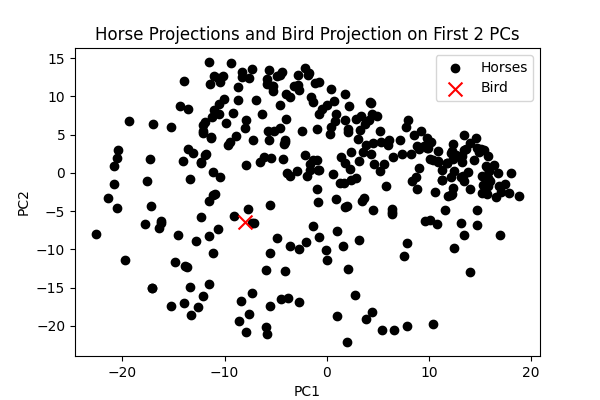
\includegraphics[width=.6\textwidth]{horse_bird_projection.png}
    \caption{Horse and Bird Image Projections on the First Two Principal Components}
    \label{fig:horse_bird_projection}
\end{figure}
\newpage
\subsubsection*{d) Reconstructing a Horse Image Using 32 Principal Components}

We reconstruct one of the horse images, \texttt{horse070.png}, using the first 32 principal components. The reconstruction is then thresholded at 0.5 to create a binary image:

\begin{minted}[fontsize=\small,frame=single]{python}
horse070_img = Image.open('horses/horse070.png').convert('L')
horse070_array = np.asarray(horse070_img, dtype=float) / 255.0
horse070_vector = horse070_array.flatten()

# Center the horse070 image
horse070_centered = horse070_vector - mean_horse

# Reconstruct using first 32 PCs
num_pcs = 32
pcs_32 = V[:, :num_pcs]
scores_32 = horse070_centered.dot(pcs_32)
horse070_reconstructed = mean_horse + scores_32.dot(pcs_32.T)
horse070_reconstructed_binary = (horse070_reconstructed > 0.5).astype(float)

# Display the original and reconstructed binary images
fig, axs = plt.subplots(1, 2, figsize=(8,4))
axs[0].imshow(horse070_array.reshape(128,128), cmap='gray')
axs[0].set_title('Original Horse070')
axs[0].axis('off')
axs[1].imshow(horse070_reconstructed_binary.reshape(128,128), cmap='gray')
axs[1].set_title('Binary Reconstruction (32 PCs)')
axs[1].axis('off')
plt.show()
\end{minted}

\begin{figure}[h]
    \centering
    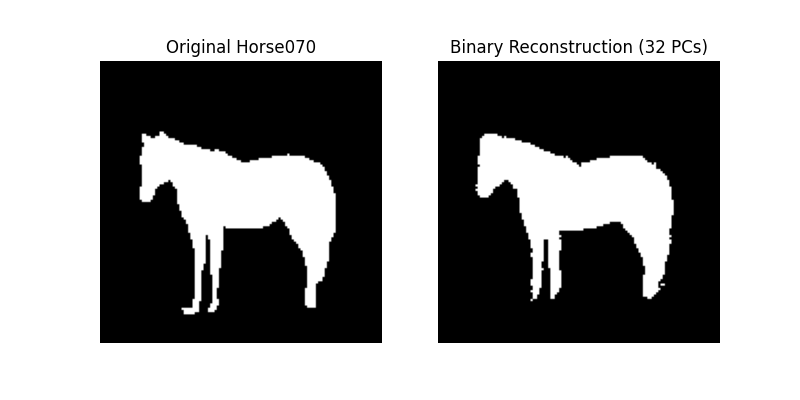
\includegraphics[width=.8\textwidth]{horse070_reconstruction.png}
    \caption{Original Horse070 (left) and Binary Reconstruction Using 32 PCs (right)}
    \label{fig:horse070_reconstruction}
\end{figure}

\subsubsection*{e) Reconstructing the Bird Image Using 32 Principal Components}

We also reconstruct the bird image using the horse PCA model and the first 32 principal components. The reconstructed image is thresholded at 0.5 to create a binary image:

\begin{minted}[fontsize=\small,frame=single]{python}
bird_reconstructed = mean_horse + (bird_centered.dot(pcs_32)).dot(pcs_32.T)
bird_reconstructed_binary = (bird_reconstructed > 0.5).astype(float)

# Display the original and reconstructed binary bird images
fig, axs = plt.subplots(1, 2, figsize=(8,4))
axs[0].imshow(bird_array.reshape(128,128), cmap='gray')
axs[0].set_title('Original Bird')
axs[0].axis('off')
axs[1].imshow(bird_reconstructed_binary.reshape(128,128), cmap='gray')
axs[1].set_title('Binary Reconstruction (32 PCs)')
axs[1].axis('off')
plt.show()
\end{minted}

\begin{figure}[h]
    \centering
    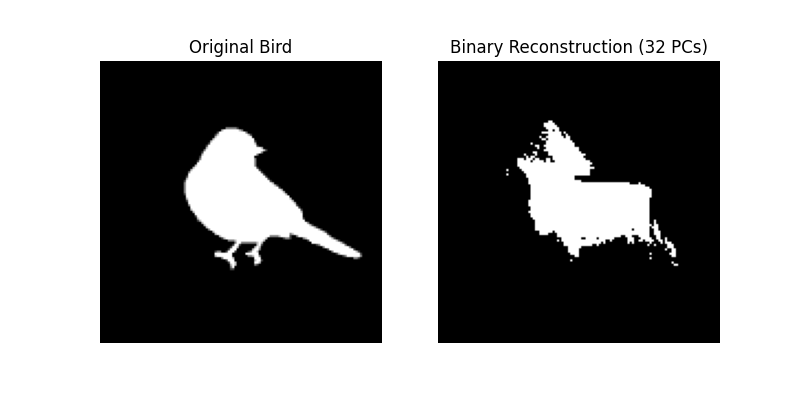
\includegraphics[width=.8\textwidth]{bird_reconstruction.png}
    \caption{Original Bird (left) and Binary Reconstruction Using 32 PCs (right)}
    \label{fig:bird_reconstruction}
\end{figure}

\subsubsection*{f) Distances to the 32-PC Plane}

We compute the distances of both the horse images and the bird image to the plane generated by the 32 largest principal components. We then plot these distances on the y-axis against the second principal component projection on the x-axis:

\begin{minted}[fontsize=\small, frame=single,breaklines]{python}
reconstructing each image using 32 PCs.
horse_reconstructions_32 = mean_horse + (horses_centered.dot(pcs_32)).dot(pcs_32.T)
distances_horses = np.linalg.norm(horses_centered - (horse_reconstructions_32 - mean_horse), axis=1)
distance_bird = np.linalg.norm(bird_centered - (bird_reconstructed - mean_horse))

# On the same graph, plot the computed distances vs the coordinates of the projections on the second PC
plt.figure(figsize=(6,4))
plt.scatter(horse_projections[:,1], distances_horses, c='black', label='Horses')
plt.scatter(bird_projection[1], distance_bird, c='red', marker='x', s=100, label='Bird')
plt.title('Distances vs. Projection on 2nd PC')
plt.xlabel('Projection on PC2')
plt.ylabel('Distance to 32-PC Plane')
plt.legend()
plt.show()
\end{minted}

\begin{figure}[ht]
    \centering
    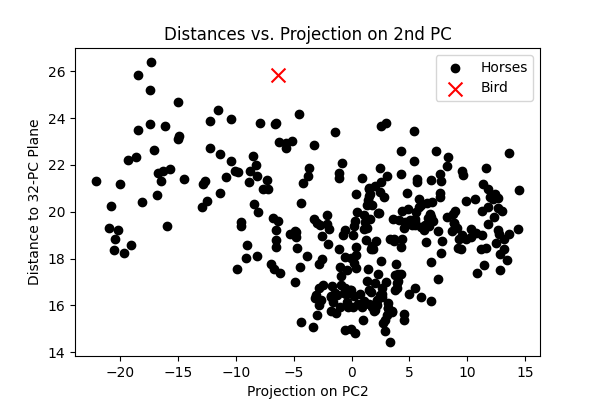
\includegraphics[width=.6\textwidth]{distances_vs_pc2.png}
    \caption{Distances to the 32-PC Plane vs. Projection on PC2 for Horses (black) and Bird (red)}
    \label{fig:distances_vs_pc2}
\end{figure}
\newpage
\subsubsection*{g) Histogram of Distances for Horses}

We plot a histogram of the distances of the horse images to the plane generated by the 32 largest PCs to understand the distribution of these distances:

\begin{minted}[fontsize=\small,frame=single,breaklines]{python}
# Plot the histogram of the distances obtained at f) for the horses
plt.figure(figsize=(6,4))
plt.hist(distances_horses, bins=20, color='black')
plt.title('Histogram of Distances to 32-PC Plane for Horses')
plt.xlabel('Distance')
plt.ylabel('Frequency')
plt.show()
\end{minted}

\begin{figure}[ht]
    \centering
    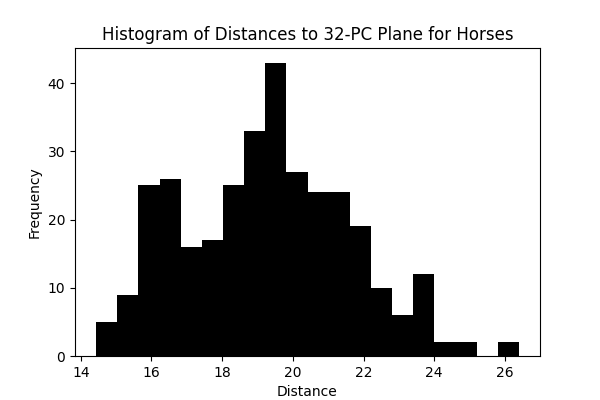
\includegraphics[width=.6\textwidth]{hist_distances_horses.png}
    \caption{Histogram of Distances to the 32-PC Plane for Horses}
    \label{fig:hist_distances_horses}
\end{figure}

\newpage
\section*{Appendix: Code}

\begin{minted}[fontsize=\small, breaklines, frame=single]{python}
import numpy as np
import matplotlib.pyplot as plt
from PIL import Image
import glob
import os

# 1. Load the horse images and bird image
# Assuming 'horses' directory contains horse images named 'horse001.png' to 'horse327.png'
horse_images_path: list[str] = sorted(glob.glob('horses/*.png'))
bird_image_path = 'bird.png'

horses: list[np.ndarray] | np.ndarray = []
for img_path in horse_images_path:
    img: Image.Image = Image.open(img_path).convert('L')
    # Normalize pixel values to [0,1]
    img_array = np.asarray(img, dtype=float) / 255.0
    horses.append(img_array.flatten())
horses = np.array(horses)  # shape: (327, 128*128)

bird_img: Image.Image = Image.open(bird_image_path).convert('L')
bird_array = np.asarray(bird_img, dtype=float) / 255.0
bird_vector:np.ndarray = bird_array.flatten()  # Flatten bird image

# 2. Compute the mean of the horse dataset
mean_horse:np.ndarray = np.mean(horses, axis=0)

# 3. Center the horse data by subtracting the mean
horses_centered = horses - mean_horse

# 4. Perform SVD on the horse images (PCA)
U, S, VT = np.linalg.svd(horses_centered, full_matrices=False)
V = VT.T  # Principal components (eigenvectors)

# a) Discard the two largest singular values and plot the remaining singular values
# discard the first two largest singular values
remaining_singular_values:np.ndarray = S[2:]
plt.figure(figsize=(6, 4))
plt.plot(remaining_singular_values, marker='o')
plt.title('Remaining Singular Values (Sorted in Decreasing Order)')
plt.xlabel('Index')
plt.ylabel('Singular Value')
plt.savefig('remaining_singular_values.png')
plt.show()

# b) Project the horses onto the first two principal components and plot
pcs:np.ndarray = V[:, :2]  # first two principal components
horse_projections:np.ndarray = horses_centered.dot(pcs)  # shape: (327, 2)

plt.figure(figsize=(6, 4))
plt.scatter(horse_projections[:, 0],
            horse_projections[:, 1], c='black', label='Horses')
plt.title('Projection of Horses onto First 2 PCs')
plt.xlabel('PC1')
plt.ylabel('PC2')
plt.legend()
plt.savefig('horse_projections.png')  # Save plot
plt.show()

# c) On the same graph, plot the horse projections in black and bird projection in red 'x'
bird_centered = bird_vector - mean_horse
bird_projection:np.ndarray = bird_centered.dot(pcs)

plt.figure(figsize=(6, 4))
plt.scatter(horse_projections[:, 0],
            horse_projections[:, 1], c='black', label='Horses')
plt.scatter(bird_projection[0], bird_projection[1],
            c='red', marker='x', s=100, label='Bird')
plt.title('Horse Projections and Bird Projection on First 2 PCs')
plt.xlabel('PC1')
plt.ylabel('PC2')
plt.legend()
plt.savefig('horse_bird_projection.png')  # Save plot
plt.show()

# d) Using the model, display the image 'horse070.png' and its binary reconstruction using 32 PCs (threshold 0.5)
# Find the horse070 image vector
horse070_img: Image.Image = Image.open('horses/horse070.png').convert('L')
horse070_array = np.asarray(horse070_img, dtype=float) / 255.0
horse070_vector:np.ndarray = horse070_array.flatten()

# Center the horse070 image
horse070_centered = horse070_vector - mean_horse

# Reconstruct using first 32 PCs
num_pcs = 32
pcs_32:np.ndarray = V[:, :num_pcs]
scores_32:np.ndarray = horse070_centered.dot(pcs_32)
horse070_reconstructed:np.ndarray = mean_horse + scores_32.dot(pcs_32.T)
horse070_reconstructed_binary:np.ndarray = (
    horse070_reconstructed > 0.5).astype(float)

# Display the original and reconstructed binary images
fig, axs = plt.subplots(1, 2, figsize=(8, 4))
axs[0].imshow(horse070_array.reshape(128, 128), cmap='gray')
axs[0].set_title('Original Horse070')
axs[0].axis('off')
axs[1].imshow(horse070_reconstructed_binary.reshape(128, 128), cmap='gray')
axs[1].set_title('Binary Reconstruction (32 PCs)')
axs[1].axis('off')
plt.savefig('horse070_reconstruction.png')  # Save figure
plt.show()

# e) Using the same model, display the bird image and its binary reconstruction using 32 PCs
bird_reconstructed:np.ndarray = mean_horse + (bird_centered.dot(pcs_32)).dot(pcs_32.T)
bird_reconstructed_binary:np.ndarray = (bird_reconstructed > 0.5).astype(float)

# Display the original and reconstructed binary bird images
fig, axs = plt.subplots(1, 2, figsize=(8, 4))
axs[0].imshow(bird_array.reshape(128, 128), cmap='gray')
axs[0].set_title('Original Bird')
axs[0].axis('off')
axs[1].imshow(bird_reconstructed_binary.reshape(128, 128), cmap='gray')
axs[1].set_title('Binary Reconstruction (32 PCs)')
axs[1].axis('off')
plt.savefig('bird_reconstruction.png')  # Save figure
plt.show()

# f) Compute the distances of the horses and the bird to the plane generated by the 32 largest PCs.
# The plane generated by the 32 largest PCs can be approximated by reconstructing each image using 32 PCs.
horse_reconstructions_32 = mean_horse + \
    (horses_centered.dot(pcs_32)).dot(pcs_32.T)
distances_horses = np.linalg.norm(
    horses_centered - (horse_reconstructions_32 - mean_horse), axis=1)
distance_bird = np.linalg.norm(
    bird_centered - (bird_reconstructed - mean_horse))

# On the same graph, plot the computed distances vs the coordinates of the projections on the second PC
plt.figure(figsize=(6, 4))
plt.scatter(horse_projections[:, 1],
            distances_horses, c='black', label='Horses')
plt.scatter(bird_projection[1], distance_bird,
            c='red', marker='x', s=100, label='Bird')
plt.title('Distances vs. Projection on 2nd PC')
plt.xlabel('Projection on PC2')
plt.ylabel('Distance to 32-PC Plane')
plt.legend()
plt.savefig('distances_vs_pc2.png')  # Save plot
plt.show()

# g) Plot the histogram of the distances obtained at f) for the horses
plt.figure(figsize=(6, 4))
plt.hist(distances_horses, bins=20, color='black')
plt.title('Histogram of Distances to 32-PC Plane for Horses')
plt.xlabel('Distance')
plt.ylabel('Frequency')
plt.savefig('hist_distances_horses.png')  # Save plot
plt.show()
\end{minted}

\end{document}
